\chapter{Současný stav řešené problematiky}
\label{sec:Theory}\

V této kapitole bude popsán stav problematiky automatického řízení a pohybových
senzorů. Konkretně bude popsaná práce \uv{Krokoměr s mikropočítačem ARM}\cite{krokomer} Šigurda Filipa, který používá ve své práce akcelerometry. Následné
budou popsaný práci \uv{Autonomní řízení auta - optimalizace detekce dráhy}\cite{draha} i \uv{Mechanizmy řízení robotického auta NXP (FREESCALE)}\cite{robot},
které popisuje autonomní řízení na základe řádkové kamery a senzorů. Autoři jsou
Vojtěch Ihn a Richard Zvonek.

\section{Krokoměr s mikropočítačem ARM}\

Tato práce se zabývala vývojem krokoměru s využitím desky NXP FRDM-K64F, která je
založená na jádře ARM© Cortex®-M4. Hlavním cílem práce bylo vytvoření krokoměru,
který by byl schopen detekovat a počítat kroky uživatele.

V práci byly vybírány různé MEMS akcelerometry podle několika kritérií: možnosti
integrace na plošný spoj, cenové dostupnosti, schopnosti komunikovat s
mikrokontrolérem prostřednictvím rozhraní $I^2C$ nebo SPI, přičemž byly vybírány
výhradně tříosé akcelerometry.

Akcelerometry byly následně testovány v různých prostředích a podmínkách, které
zahrnovaly chůzi po~rovině, po trávě, do a z kopce, a také chůzi do a ze schodů.

Každé měření bylo doprovázeno dvěma krokoměry:  Xiaomi Mi Band a aplikace
\uv{Pedometer} provozovanou na mobilním telefonu Nokia 6.1. Výsledky jednotlivých
akcelerometrů v~jednotlivých situacích byli velice podobné:

\begin{table}[!h]
	\centering
	\begin{tabular}{lccc}
		\toprule
		Měření s akcelerometrem      & délka chůze & Xiaomi Mi Band & Nokia 6.1 \\
		\midrule
		NXP FXOS8700CQ               & 3m 35s      & 345            & 351       \\
		NXP MMA8452Q                 & 3m 25s      & 339            & 337       \\
		Analog Devices ADXL345       & 3m 31s      & 343            & 339       \\
		STMicroelectronics LSM303DLH & 3m 30s      & 338            & 336       \\
		\bottomrule
	\end{tabular}
	\caption{Počet kroků při chůzi do kopce s krokoměrem v ruce\cite{krokomer}.}
	\label{tab:1}
\end{table}

Dále byly otestovány a porovnány různé filtry pro odstranění šumu z naměřených dat.
Použity byly filtry typu dolní propust, a to z důvodu, že normální chůze
nepřekračuje rychlost čtyř kroků za~sekundu, což znamená, že frekvence vyšší než
4~Hz byly považovány za šum. Filtrace signálu byla prováděna pomoci filtrů s
konečnou impulzní odezvou (FIR) a s nekonečnou impulzní odezvou~(IIR).

\begin{figure}[!h]
	\centering
	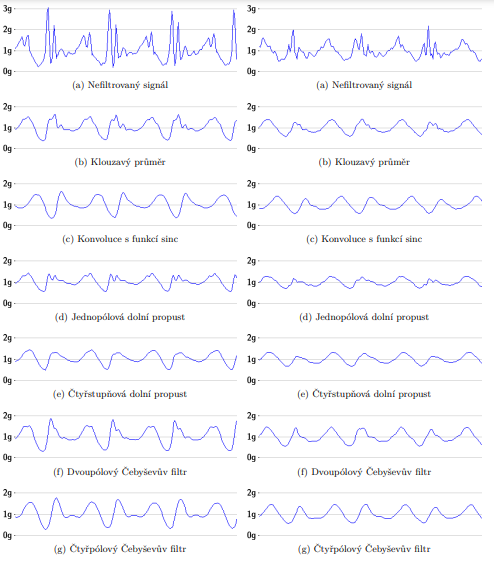
\includegraphics[width = .95\linewidth]{Figures/Filtry.png}
	\captionsetup{justification = centering}
	\caption{Čtyřsekundové ukázky aplikovaných filtrů. Vlevo: chůze po rovině s
	akcelerometrem v~kapse. Vpravo: chůze do kopce s akcelerometrem v
	kapse\cite{krokomer}.}
	\label{fig:filtr}
\end{figure}

Po porovnání filtrů byl jako nejlepší vyhodnocen dvoupólový Čebyševův filtr, který
ve srovnání s ostatními je výpočetně méně náročný a odstranil velké množství šumu se
zachováním amplitudy signálu. Výsledky aplikace filtrů jsou zobrazeny na obrázku \ref{fig:filtr}.

Pro počítání kroků byly implementovány dva způsoby detekce kroků. První z nich se
ukázal jako nevyhovující. Druhý způsob detekce kroků byl o poznáni přesnější.
Algoritmus funguje na principu stavového automatu, který má 2 stavy pro hledání
nástupních a sestupných hran.

Závěrečné testování kompletního řešení proběhlo chůzi po městě. Trasa byla přibližně
1650~metrů dlouhá. Výsledky měření byly porovnány s komerčně dostupnými krokoměry
pro ověření přesnosti navrženého řešení. Tabulka \ref{tab:2}  zobrazuje počty
naměřených kroků jednotlivými krokoměry.

Testování ukázalo, že výsledky jsou velmi podobné výsledkům ostatních dvou
krokoměrů\cite{krokomer}.

\begin{table}[!h]
	\centering
	\begin{tabular}{lcccc}
		\toprule
		Umístění krokoměru & délka chůze & Xiaomi Mi Band & Nokia 6.1 & FRDM-K64F \\
		\midrule
		V kapse            & 18m 46s     & 1986           & 2013      & 2021      \\
		V ruce             & 18m 36s     & 1993           & 2007      & 2010      \\
		\bottomrule
	\end{tabular}
	\caption{Počet kroků při závěrečném měření\cite{krokomer}.}
	\label{tab:2}
	\vspace{-10pt}
\end{table}

\section{Autonomní řízení auta - optimalizace detekce dráhy}\

Tato práce se zaměřila na zpracování obrazu získaného z řádkové kamery a na následné
vyhledávání okrajových čar dráhy s využitím různých typů objektivů a filtrů. Cílem
bylo najít optimální kombinaci, která by umožňovala nejpřesnější detekci dráhy pro
autonomní řízení vozidla. Pro dosažení tohoto cíle práce zkoumala různé metody a
techniky zpracování obrazu, včetně výběru a testování objektivů kamery, aplikaci
filtrů pro zlepšení kvality obrazu a implementaci algoritmů pro~efektivní detekci
dráhy.

Finální výběr kamery a objektivu byl založen na schopnosti kamer efektivně detekovat
okrajové čáry za různých světelných podmínek.

Dále byly otestovány různé kombinace filtrů pro redukci šumu, detekci hran a
prahování. Ve~výsledku byly pro implementaci vybrány 4 filtry: mediánový filtr,
Gaussův filtr, morfologický gradient a Otsu prahování.

Algoritmus byl testován při umělém osvětlení i při denním světle. Při rovnoměrném
umělém osvětlení byla detekce okrajových čar na dráze spolehlivá. Při denním světle
byly dosaženy slušné výsledky, které avšak nešlo považovat za ideální\cite{draha}.

\section{Mechanizmy řízení robotického auta NXP (FREESCALE)}\

V rámci této práce byl vyvinut softwarový systém pro robotický model auta. Systém
byl navržen tak, aby umožňoval autonomní navigaci po závodní dráze s využitím dat
získaných z řádkové kamery a dalších senzorů. Řídící software se skládal ze dvou
hlavních částí: zpracování obrazu z řádkové kamery a řízení na základě získaných
informací z obrazu.

Pro zpracování obrazu byly použitý: filtrování mediánem pro odstranění šumu,
normalizace obrazu pro přizpůsobení světelným podmínkám a prahování průměrem.

Pro řízení pomocí dat z kamery byl software schopen detekovat okraje dráhy a na
základě této informace řídit směr a rychlost auta. Klíčovým prvkem bylo efektivní
využití PID regulátoru.

Práce rovněž zahrnovala vývoj a integraci různých senzorů, včetně IMU a IR senzorů.
IMU~jednotka byla použita k detekci zastavení vozidla, zatímco infračervené senzory
sloužily k detekci blízkých objektů a překážek.

Následně bylo robotické auto testováno na soutěži NXP Cup, kde úspěšně zvládlo
všechny tři dodatečné disciplíny v kvalifikačním kole\cite{robot}.

\endinput
